\PassOptionsToPackage{quiet}{fontspec}
\documentclass[12pt,a4paper,UTF8]{article}
\usepackage{thesis} % 格式控制
\usepackage{indentfirst}
\usepackage{enumitem}
\usepackage{amsmath} % 数学公式支持
\usepackage{amsfonts} % 数学字体支持
\usepackage{amssymb} % 数学符号支持
\usepackage{graphicx} % 图片插入支持
\usepackage{float} % 浮动体位置控制，支持 [H] 选项
\usepackage{caption} % 图表标题格式控制
\usepackage{geometry} % 页面布局控制
\usepackage{setspace} % 行距控制
\usepackage{xeCJK} % 中文字体支持
\usepackage{fontspec} % 字体设置
\usepackage[most]{tcolorbox} % 高亮按键命令
\setlength{\parindent}{2em} % 控制首行缩进  
\addtolength{\parskip}{3pt} % 控制段落距离  
\onehalfspacing % 1.5倍行距  
\graphicspath{{./figures/}} % 指定图片所在文件夹  
\setCJKmainfont{SimSun}
\setCJKfamilyfont{hei}{SimHei} 

\classname{\heiti\bfseries 人工智能实验}  % 设置课程名称
\makepagestyle{}{}

\newtcbox{\keyblue}{on line,
  colframe=blue!60!black, colback=blue!10,
  boxrule=0.8pt, arc=2pt, boxsep=0pt, left=2pt, right=2pt, top=1pt, bottom=1pt,
  tcbox raise base, fontupper=\color{blue}\bfseries}

\begin{document}
\maketitlepage{实验1-1 分类模型}{玉泉高分子楼-203}{郑智瑄}{3230103913}{\today}{魏准} %封面页 

\maketoc

\section{\heiti\bfseries 实验目的}
\begin{enumerate}
    \item 掌握快速加法器的设计方法。
    \item 熟悉流水线技术。
    \item 掌握时序仿真的工作流程
\end{enumerate}

\section{\heiti\bfseries 实验任务}
\begin{enumerate}
    \item 采用"进位选择加法"技术设计 32 位加法器，并对设计进行功能仿真和时序仿真。
    \item 采用四级流水线技术设计 32 位加法器，并对设计进行功能仿真和时序仿真。
\end{enumerate}

\section{\heiti\bfseries 实验设备}

装有 Vivado、ModelSim SE 软件的计算机。

\section{\heiti\bfseries 提供的代码}

\begin{enumerate}
    \item 4 位加法器测试代码 adder\_4bits\_tb.v。
    \item 32 位进位选择加法器测试代码 adder\_32bits\_tb.v。
    \item 32 位流水线加法器测试代码 pipeline\_adder\_tb.v。
\end{enumerate}

\section{\heiti\bfseries 实验内容}

\begin{enumerate}
    \item 编写 4 位先行进位加法器的 Verilog HDL 代码，并用 ModelSim 软件进行功能仿真。
    \item 32 位进位选择加法器的设计
    \begin{enumerate}[label=(\arabic*)]
        \item 编写用 32 位进位选择加法器的 Verilog HDL 代码，并用 ModelSim 软件进行功能。
        \item 对 32 位加法器进行时序仿真
    \end{enumerate}
    \item 编写采用4级流水线技术的32位加法器的Verilog HDL代码，并对设计进行时序仿真。
\end{enumerate}

\section{\heiti\bfseries 实验过程与结果}

\subsection{\heiti\bfseries 4位先行进位加法器}

\subsubsection{\heiti\bfseries 设计原理}

两个加数分别为 $A_3A_2A_1A_0$ 和 $B_3B_2B_1B_0$，$C_{-1}$ 为最低位进位。设两个辅助变量分别为 $G_3G_2G_1G_0$ 和 $P_3P_2P_1P_0$；$G_i = A_i \& B_i$、$P_i = A_i + B_i$。

一位全加器的逻辑表达式可转化为
\begin{equation}
\begin{cases}
S_i = P_i \overline{G_i} \oplus C_{i-1} \\
C_i = G_i + P_i C_{i-1}
\end{cases}
\end{equation}

利用上述关系，一个四位加法器的进位计算就变转化为
\begin{equation}
\begin{cases}
C_0 = G_0 + P_0 C_{-1} \\
C_1 = G_1 + P_1 C_0 = G_1 + P_1 G_0 + P_1 P_0 C_{-1} \\
C_2 = G_2 + P_2 C_1 = G_2 + P_2 G_1 + P_2 P_1 G_0 + P_2 P_1 P_0 C_{-1} \\
C_3 = G_3 + P_3 C_2 = G_3 + P_3 G_2 + P_3 P_2 G_1 + P_3 P_2 P_1 G_0 + P_3 P_2 P_1 P_0 C_{-1}
\end{cases}
\end{equation}

由式（5.13）可以看出，每一个进位的计算都直接依赖于整个加法器的最初输入，而不需要等待相邻低位的进位传递。理论上，每一个进位的计算都只需要三个门延迟时间，即产生 $G[i]$、$P[i]$ 的与门和或门，输入为 $G[i]$、$P[i]$、$C_{-1}$ 的与门，以及最终的或门。同样道理，理论上最终结果 sum 的得到只需要四个门延迟时间。

实际上，当加数位数较大时，输入需要驱动的门数量较多，其 VLSI 实现的输出时延增加很多，考虑到互连线的延时情况将会更加糟糕。因此，通常在芯片实现时先设计位数较少的超前进位加法器结构，而后以此为基本结构来构造位数较大的加法器。
\subsubsection{\heiti\bfseries Verilog HDL 代码与设计分析}

\begin{enumerate}
    \item {\heiti\bfseries 模块接口：}
    \begin{itemize}
    \item a,b:4 位输入信号，两个需要相加的 4 位二进制数。
    \item ci(carry in):进位输入，低位加法器的进位。
    \item s(sum):4 位的和输出。
    \item co(carry out):进位输出，最高位的进位。
    \end{itemize}
    \item {\heiti\bfseries 内部信号：}
    \begin{itemize}
    \item g(generate):生成进位
    \item p(propagate):传播进位
    \item c(carry):内部进位，存储每个位的进位值。
    \end{itemize}
    \item {\heiti\bfseries 部分电路图(注：标注与实验原理中有所不同)：}
    \begin{figure}[H]
    \centering
    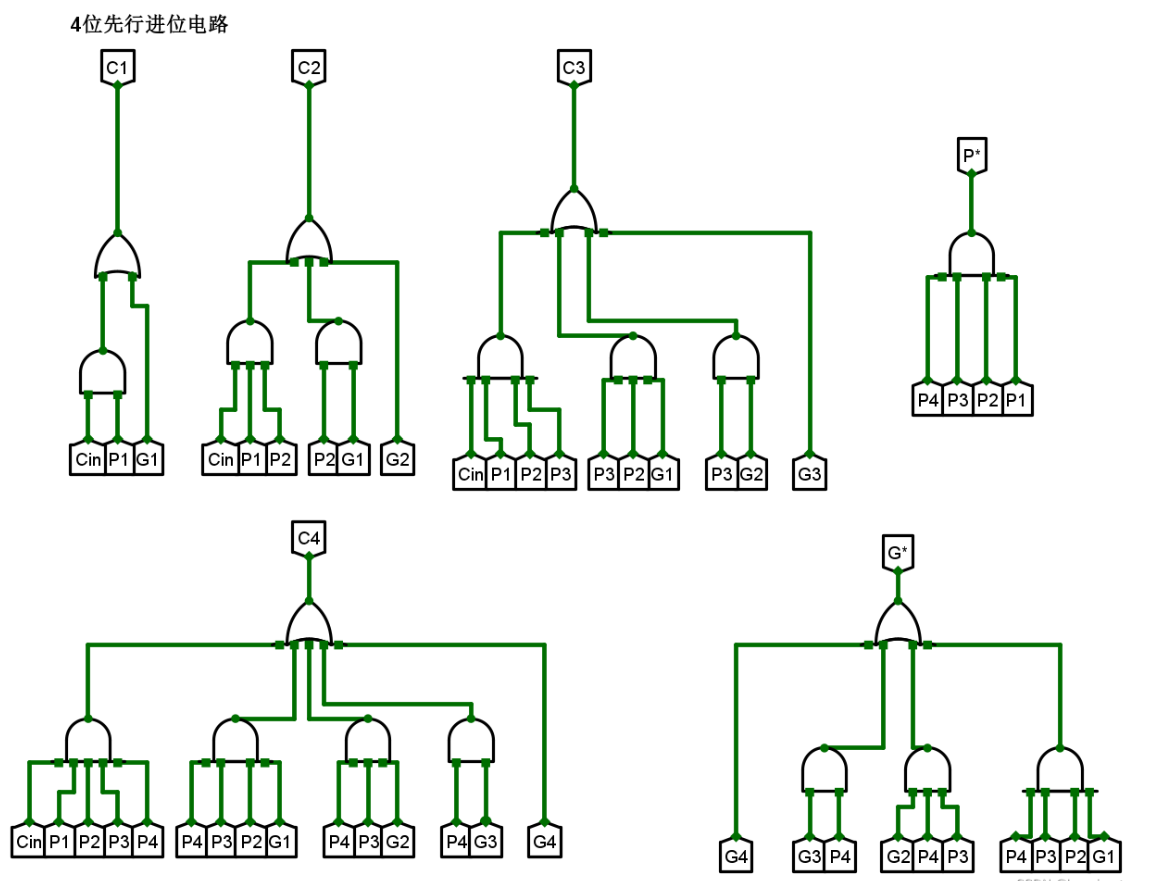
\includegraphics[width=1\textwidth]{p6.png}
    \caption{4 位先行进位加法器 ModelSim仿真结果}
    \end{figure}

\end{enumerate}


\clearpage

\begin{lstlisting}[language=verilog, caption=4位先行进位加法器 Verilog HDL 代码, label=lst:adder_4bits]
module adder_4bits(
    input  [3:0] a,
    input  [3:0] b,
    input  ci,
    output [3:0] s,
    output co
);

    wire [3:0] g;  // 进位生成信号 (Generate)
    wire [3:0] p;  // 进位传播信号 (Propagate)
    wire [2:0] c;  // 中间进位信号

    // 计算进位生成和传播信号
    assign g = a & b;
    assign p = a | b;

    // 超前进位逻辑
    assign c[0] = g[0] | (p[0] & ci);
    assign c[1] = g[1] | (p[1] & g[0]) | (p[1] & p[0] & ci);
    assign c[2] = g[2] | (p[2] & g[1]) | (p[2] & p[1] & g[0]) | (p[2] & p[1] & p[0] & ci);
    assign co = g[3] | (p[3] & g[2]) | (p[3] & p[2] & g[1]) | (p[3] & p[2] & p[1] & g[0]) | (p[3] & p[2] & p[1] & p[0] & ci);

    // 计算和
    assign s[0] = (p[0] & ~g[0]) ^ ci;
    assign s[1] = (p[1] & ~g[1]) ^ c[0];
    assign s[2] = (p[2] & ~g[2]) ^ c[1];
    assign s[3] = (p[3] & ~g[3]) ^ c[2];

endmodule
\end{lstlisting}

\subsubsection{\heiti\bfseries ModelSim 仿真与结果分析}

\begin{figure}[H]
    \centering
    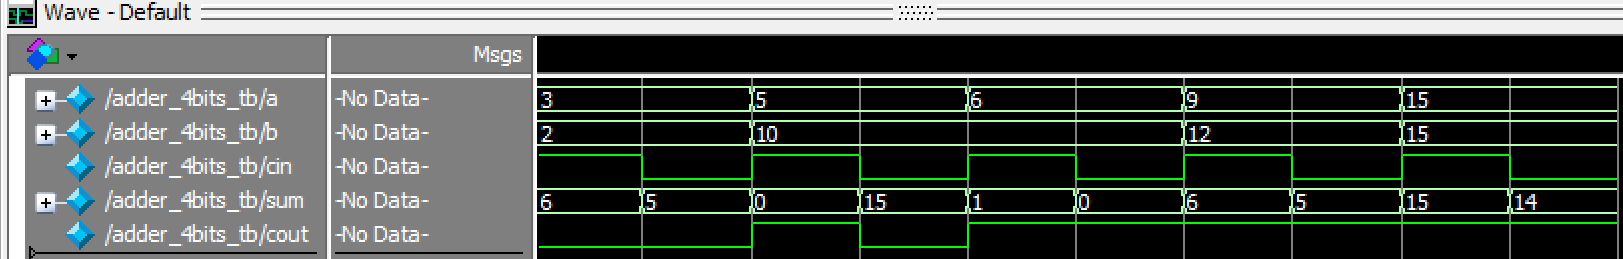
\includegraphics[width=1\textwidth]{p3.png}
    \caption{4 位先行进位加法器 ModelSim仿真结果}
\end{figure}

【实验结果】:仿真结果表示，4 位先行进位加法器功能正常。

\subsection{\heiti\bfseries 32 位进位选择加法器}

\subsubsection{\heiti\bfseries 设计原理}

实际上，由超前进位加法器级联构成的多位加法器只是提高了进位传递的速度，其计算过程与行波进位加法器同样需要等待进位传递的完成。

借鉴并行计算的思想，人们提出了进位选择加法器结构，或者称为有条件的加法器结构（conditional sum adder），其算法的实质是增加硬件面积换取速度性能的提高。二进制加法的特点是进位或者为逻辑1，或者为逻辑0，二者必居其一。将进位链较长的加法器分为 $M$ 块，分别进行加法计算，对除去最低位计算块外的 $M - 1$ 块加法结构复制两份，其进位输入分别预定为逻辑1和逻辑0。于是，$M$ 块加法器可以同时并行进行各自的加法运算，然后根据各自相邻低位加法运算结果产生的进位输出，选择正确的加法结果输出。图5.6所示为12位进位选择加法器的逻辑结构图。12位加法器划分为3块，最低一块（4位）由4位超前进位加法器直接构成，后两块分别假设前一块的进位为0或1将两种结果都计算出来，再根据前级进位选择正确的和与进位。如果每一块加法结构内部都采用速度较快的超前进位加法器结构，那么进位选择加法器的计算时延为

\begin{equation}
t_{CSA} = t_{carry} + (M - 2)t_{MUX} + t_{sum}
\end{equation}

其中，$t_{sum}$、$t_{carry}$ 分别为加法器的和与加法器的进位时延，$t_{MUX}$ 为数据选择器的时延。

\begin{figure}[H]
    \centering
    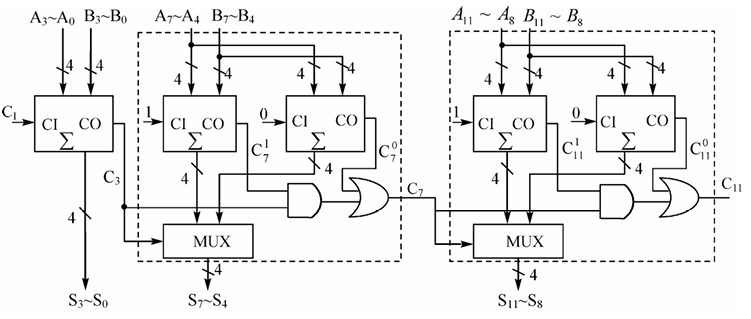
\includegraphics[width=0.8\textwidth]{p1.png}
    \caption{12位进位选择加法器原理图}
\end{figure}

\subsubsection{\heiti\bfseries Verilog HDL 代码与设计分析}

\begin{enumerate}
    \item {\heiti\bfseries 模块接口：}
    \begin{itemize}
    \item a,b:32 位输入信号，表示两个需要相加的 32 位二进制数。
    \item ci(carry in):进位输入，低位加法器的进位。
    \item s(sum):32 位的和输出，表示加法结果。
    \item co(carry out):进位输出，表示最高位的进位。
    \end{itemize}
    \item {\heiti\bfseries 内部信号：}
    \begin{itemize}
    \item c1$\sim$c7:各 4 位段之间的进位信号，用于连接 8 个 4 位加法器模块。
    \item s0\_0, s0\_1, $\ldots$, s7\_0, s7\_1:每个 4 位段在进位为 0 和进位为 1 时的两种可能的和结果。
    \item co0\_0, co0\_1, $\ldots$, co7\_0, co7\_1:每个 4 位段在进位为 0 和进位为 1 时的两种可能的进位输出。
    \end{itemize}
    \item {\heiti\bfseries 设计思路：}
    \begin{itemize}
    \item 将 32 位加法器分为 8 个 4 位段，每段使用先行进位加法器实现。
    \item 第 0 段直接使用输入进位 ci 进行计算。
    \item 第 1$\sim$7 段分别预计算进位为 0 和进位为 1 的两种结果，然后根据前一段的实际进位输出，通过二选一多路选择器选择正确的结果。
    \item 这种设计使得各段可以并行计算，大大减少了进位传播延迟，提高了运算速度。
    \end{itemize}
\end{enumerate}

\begin{lstlisting}[language=verilog, caption=32位进位选择加法器 Verilog HDL 代码, label=lst:adder_32bits]
module adder_32bits(
    input  [31:0] a,
    input  [31:0] b,
    input  ci,
    output [31:0] s,
    output co
);

    wire c1, c2, c3, c4, c5, c6, c7;  // 各4位段之间的进位信号

    // 每个4位段的两种可能结果(进位为0和进位为1时)
    wire [3:0] s1_0, s1_1, s2_0, s2_1, s3_0, s3_1, s4_0, s4_1;
    wire [3:0] s5_0, s5_1, s6_0, s6_1, s7_0, s7_1;
    wire       co1_0, co1_1, co2_0, co2_1, co3_0, co3_1, co4_0, co4_1;
    wire       co5_0, co5_1, co6_0, co6_1, co7_0, co7_1;

    // 第0段(bit[3:0]): 直接使用实际进位ci
    adder_4bits u0 (.a(a[3:0]), .b(b[3:0]), .ci(ci), .s(s[3:0]), .co(c1));

    // 第1段(bit[7:4]): 预计算进位为0和1的两种结果，根据c1选择
    adder_4bits u1_0 (.a(a[7:4]),   .b(b[7:4]),   .ci(1'b0), .s(s1_0), .co(co1_0));
    adder_4bits u1_1 (.a(a[7:4]),   .b(b[7:4]),   .ci(1'b1), .s(s1_1), .co(co1_1));
    assign s[7:4] = c1 ? s1_1 : s1_0;
    assign c2     = c1 ? co1_1 : co1_0;

    // 第2段(bit[11:8]): 根据c2选择结果
    adder_4bits u2_0 (.a(a[11:8]),  .b(b[11:8]),  .ci(1'b0), .s(s2_0), .co(co2_0));
    adder_4bits u2_1 (.a(a[11:8]),  .b(b[11:8]),  .ci(1'b1), .s(s2_1), .co(co2_1));
    assign s[11:8] = c2 ? s2_1 : s2_0;
    assign c3      = c2 ? co2_1 : co2_0;

    // 第3段(bit[15:12]): 根据c3选择结果
    adder_4bits u3_0 (.a(a[15:12]), .b(b[15:12]), .ci(1'b0), .s(s3_0), .co(co3_0));
    adder_4bits u3_1 (.a(a[15:12]), .b(b[15:12]), .ci(1'b1), .s(s3_1), .co(co3_1));
    assign s[15:12] = c3 ? s3_1 : s3_0;
    assign c4       = c3 ? co3_1 : co3_0;

    // 第4段(bit[19:16]): 根据c4选择结果
    adder_4bits u4_0 (.a(a[19:16]), .b(b[19:16]), .ci(1'b0), .s(s4_0), .co(co4_0));
    adder_4bits u4_1 (.a(a[19:16]), .b(b[19:16]), .ci(1'b1), .s(s4_1), .co(co4_1));
    assign s[19:16] = c4 ? s4_1 : s4_0;
    assign c5       = c4 ? co4_1 : co4_0;

    // 第5段(bit[23:20]): 根据c5选择结果
    adder_4bits u5_0 (.a(a[23:20]), .b(b[23:20]), .ci(1'b0), .s(s5_0), .co(co5_0));
    adder_4bits u5_1 (.a(a[23:20]), .b(b[23:20]), .ci(1'b1), .s(s5_1), .co(co5_1));
    assign s[23:20] = c5 ? s5_1 : s5_0;
    assign c6       = c5 ? co5_1 : co5_0;

    // 第6段(bit[27:24]): 根据c6选择结果
    adder_4bits u6_0 (.a(a[27:24]), .b(b[27:24]), .ci(1'b0), .s(s6_0), .co(co6_0));
    adder_4bits u6_1 (.a(a[27:24]), .b(b[27:24]), .ci(1'b1), .s(s6_1), .co(co6_1));
    assign s[27:24] = c6 ? s6_1 : s6_0;
    assign c7       = c6 ? co6_1 : co6_0;

    // 第7段(bit[31:28]): 根据c7选择结果并输出最终进位
    adder_4bits u7_0 (.a(a[31:28]), .b(b[31:28]), .ci(1'b0), .s(s7_0), .co(co7_0));
    adder_4bits u7_1 (.a(a[31:28]), .b(b[31:28]), .ci(1'b1), .s(s7_1), .co(co7_1));
    assign s[31:28] = c7 ? s7_1 : s7_0;
    assign co       = c7 ? co7_1 : co7_0;

endmodule
\end{lstlisting}
\subsubsection{\heiti\bfseries ModelSim 仿真与结果分析}

\begin{figure}[H]
    \centering
    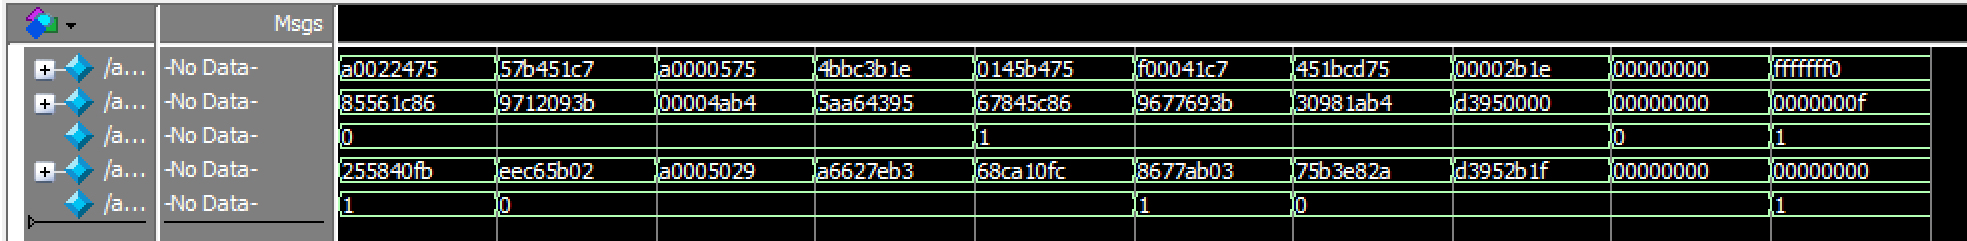
\includegraphics[width=1\textwidth]{p4.png}
    \caption{32 位进位选择加法器 ModelSim仿真结果}
\end{figure}

【实验结果】:ModelSim仿真结果表示，32 位进位选择加法器功能正常。

\subsubsection{\heiti\bfseries 时序仿真}
在vivado 中进行综合和实现后，对32位进位选择加法器进行时序仿真，仿真结果
如下，可以看到时序仿真中信号存在建立时间和毛刺等现象

\begin{figure}[H]
    \centering
    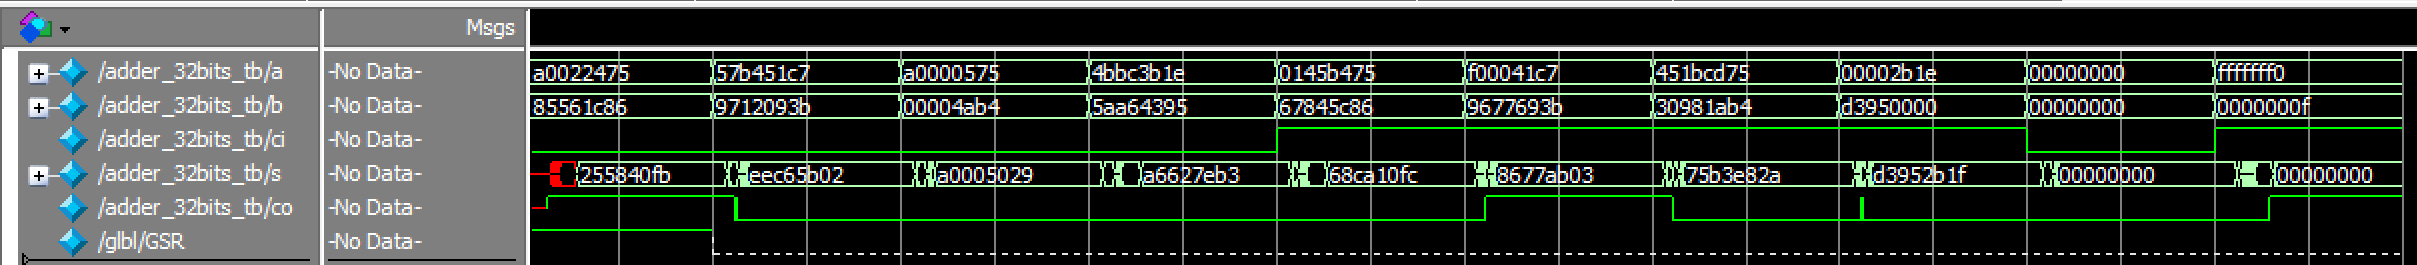
\includegraphics[width=1\textwidth]{p10.png}
    \caption{32 位进位选择加法器 时序仿真结果}
\end{figure}

【实验结果】:时序仿真结果表示，32 位进位选择加法器在考虑时序和硬件时延的情况下功能正常。

\subsection{\heiti\bfseries 32 位流水线加法器}

\subsubsection{\heiti\bfseries 设计原理}

在数字系统中，如果完成某些复杂逻辑功能需要较长的时延，就会使系统很难运行在较高的工作频率上。流水线设计（pipeline design）是经常用于提高系统运行速度的一种有效方法，即在长时延的逻辑功能块中插入触发器，将复杂的逻辑操作分步进行，减少每个部分的操作，从而提高系统的运行速度。

图5.7所示为采用4级流水线技术的32位加法器的原理框图，采用了5级锁存、4级8位加法，整个加法只受8位加法器工作速度了限制，从而提高了整个加法器工作速度。

\begin{figure}[H]
    \centering
    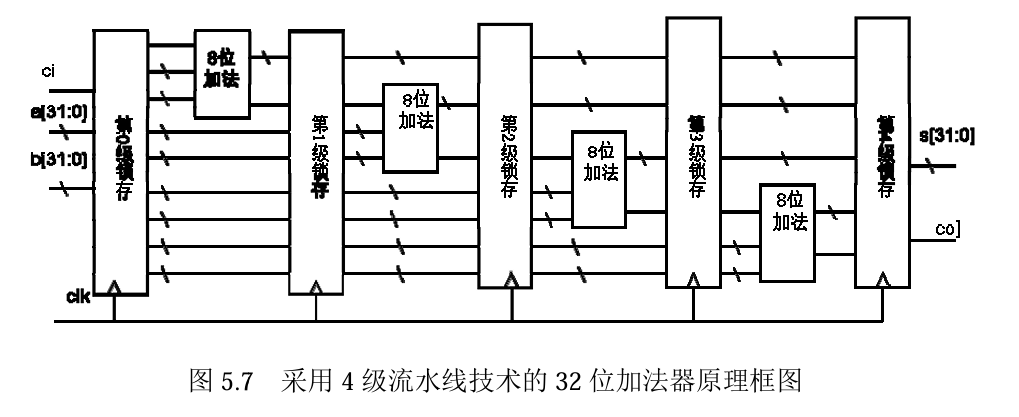
\includegraphics[width=0.8\textwidth]{p2.png}
    \caption{采用4级流水线技术的32位加法器原理框图}
\end{figure}

\subsubsection{\heiti\bfseries Verilog HDL 代码与设计分析}

\begin{enumerate}
    \item {\heiti\bfseries 模块接口：}
    \begin{itemize}
    \item clk(clock):时钟信号，用于同步流水线各级的数据传输。
    \item a,b:32 位输入信号，表示两个需要相加的 32 位二进制数。
    \item ci(carry in):进位输入，为低位加法器的进位。
    \item s(sum):32 位的和输出（寄存器类型），表示加法结果。
    \item co(carry out):进位输出（寄存器类型），表示最高位的进位。
    \end{itemize}
    \item {\heiti\bfseries 内部信号：}
    \begin{itemize}
    \item a\_reg1, b\_reg1, ci\_reg1:第 1 级流水线寄存器，用于锁存输入数据。
    \item a\_reg2[23:0], b\_reg2[23:0]:第 2 级流水线寄存器，存储剩余高 24 位数据。
    \item s0\_reg2[7:0]:第 2 级流水线寄存器，存储第 0 段（bit[7:0]）的和。
    \item c1\_reg2:第 2 级流水线寄存器，存储第 0 段产生的进位。
    \item a\_reg3[15:0], b\_reg3[15:0]:第 3 级流水线寄存器，存储剩余高 16 位数据。
    \item s0\_reg3, s1\_reg3:第 3 级流水线寄存器，存储第 0、1 段的和。
    \item c2\_reg3:第 3 级流水线寄存器，存储第 1 段产生的进位。
    \item a\_reg4[7:0], b\_reg4[7:0]:第 4 级流水线寄存器，存储剩余高 8 位数据。
    \item s0\_reg4, s1\_reg4, s2\_reg4:第 4 级流水线寄存器，存储第 0、1、2 段的和。
    \item c3\_reg4:第 4 级流水线寄存器，存储第 2 段产生的进位。
    \end{itemize}
    \item {\heiti\bfseries 设计思路：}
    \begin{itemize}
    \item 采用 5 级流水线结构，将 32 位加法分为 4 个 8 位加法段。
    \item 第 1 级：锁存输入数据 a、b、ci。
    \item 第 2 级：计算 bit[7:0] 的加法结果，同时将高 24 位数据传递到下一级。
    \item 第 3 级：计算 bit[15:8] 的加法结果，同时将高 16 位数据和 bit[7:0] 的结果传递到下一级。
    \item 第 4 级：计算 bit[23:16] 的加法结果，同时将高 8 位数据和 bit[15:0] 的结果传递到下一级。
    \item 第 5 级：计算 bit[31:24] 的加法结果，并组装完整的 32 位和与进位输出。
    \item 每个时钟周期可以接收一组新的输入数据，虽然单个数据的延迟为 5 个时钟周期，但吞吐量达到每周期一个结果（流水线填满后）。
    \end{itemize}
\end{enumerate}

\begin{lstlisting}[language=verilog, caption=32位流水线加法器 Verilog HDL 代码, label=lst:pipeline_adder]
`timescale 1ns/10ps
module pipeline_adder (
    input clk,
    input [31:0] a,
    input [31:0] b,
    input ci,
    output reg [31:0] s,
    output reg co
);

    // 第1级流水线寄存器
    reg [31:0] a_reg1, b_reg1;
    reg        ci_reg1;

    // 第2级流水线寄存器
    reg [23:0] a_reg2, b_reg2;  // 剩余高24位数据
    reg [7:0]  s0_reg2;          // 第0段(bit[7:0])的和
    reg        c1_reg2;          // 第0段产生的进位

    // 第3级流水线寄存器
    reg [15:0] a_reg3, b_reg3;  // 剩余高16位数据
    reg [7:0]  s0_reg3, s1_reg3; // 第0、1段的和
    reg        c2_reg3;          // 第1段产生的进位

    // 第4级流水线寄存器
    reg [7:0]  a_reg4, b_reg4;   // 剩余高8位数据
    reg [7:0]  s0_reg4, s1_reg4, s2_reg4;  // 第0、1、2段的和
    reg        c3_reg4;          // 第2段产生的进位

    always @(posedge clk) begin
        // --- 第1级流水线: 输入数据寄存 ---
        a_reg1  <= a;
        b_reg1  <= b;
        ci_reg1 <= ci;

        // --- 第2级流水线: 计算bit[7:0]，传递高24位 ---
        {c1_reg2, s0_reg2} <= a_reg1[7:0] + b_reg1[7:0] + ci_reg1;
        a_reg2 <= a_reg1[31:8];
        b_reg2 <= b_reg1[31:8];

        // --- 第3级流水线: 计算bit[15:8]，传递高16位和bit[7:0]结果 ---
        {c2_reg3, s1_reg3} <= a_reg2[7:0] + b_reg2[7:0] + c1_reg2;
        a_reg3 <= a_reg2[23:8];
        b_reg3 <= b_reg2[23:8];
        s0_reg3 <= s0_reg2;

        // --- 第4级流水线: 计算bit[23:16]，传递高8位和bit[15:0]结果 ---
        {c3_reg4, s2_reg4} <= a_reg3[7:0] + b_reg3[7:0] + c2_reg3;
        a_reg4 <= a_reg3[15:8];
        b_reg4 <= b_reg3[15:8];
        s1_reg4 <= s1_reg3;
        s0_reg4 <= s0_reg3;

        // --- 第5级流水线: 计算bit[31:24]，组装最终结果 ---
        {co, s[31:24]} <= a_reg4 + b_reg4 + c3_reg4;
        s[23:16] <= s2_reg4;
        s[15:8]  <= s1_reg4;
        s[7:0]   <= s0_reg4;
    end

endmodule
\end{lstlisting}
\subsubsection{\heiti\bfseries ModelSim 仿真与结果分析}

\begin{figure}[H]
    \centering
    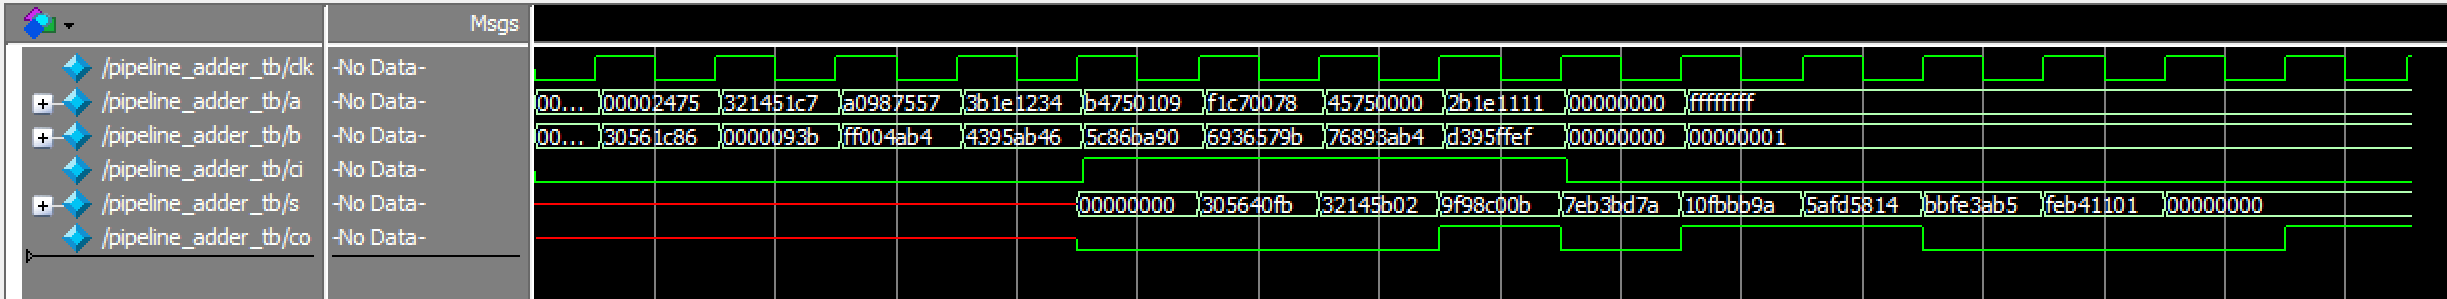
\includegraphics[width=1\textwidth]{p7.png}
    \caption{32位流水线加法器ModelSim仿真结果}
\end{figure}

【实验结果】:ModelSim仿真结果表示，设计的32位流水线加法器功能正常，在第一个数据到达后，经过四个时钟周期后，输出了正确的结果。并实现了流水线的效果。

\subsubsection{\heiti\bfseries 时序仿真与结果分析}
在vivado 中进行综合和实现后，对32位流水线加法器进行时序仿真，仿真结果如
下，可以看到时序仿真中信号存在建立时间和时钟上升沿后的时延等现象

\begin{figure}[H]
    \centering
    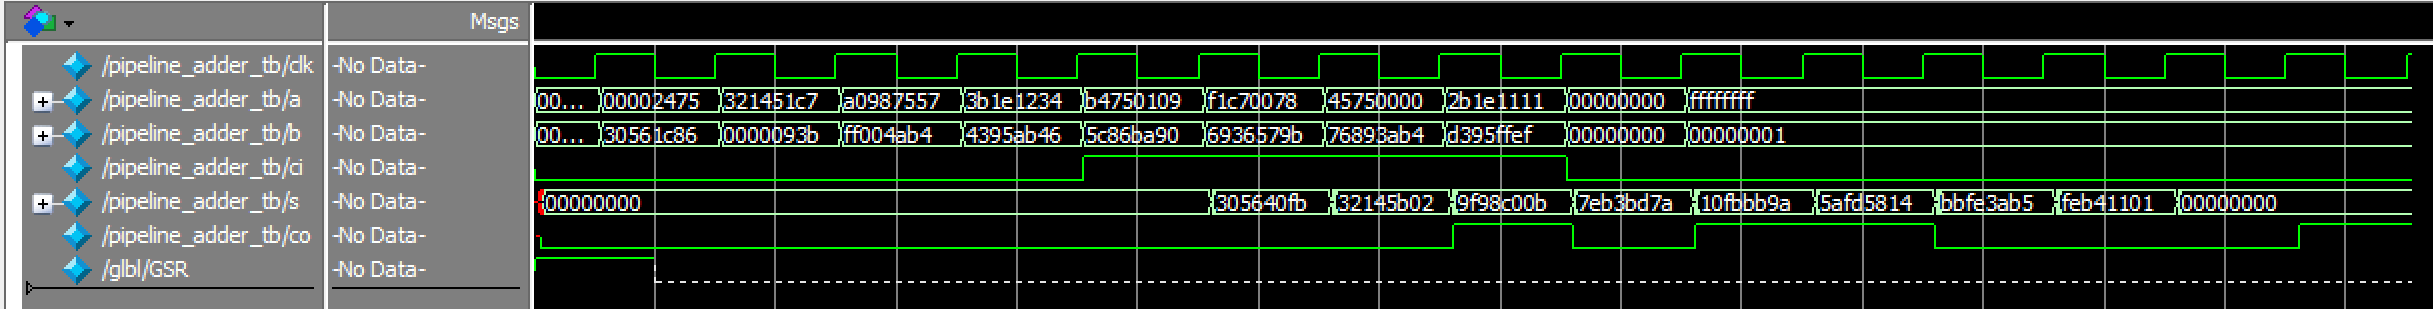
\includegraphics[width=1\textwidth]{p13.png}
    \caption{32位流水线加法器时序仿真结果}
\end{figure}

【实验结果】:时序仿真结果表示，设计的32位流水线加法器在考虑时序和硬件时延的情况下功能正常

\section{\heiti\bfseries 遇到的问题及解决方法}

在设计 32 位流水线加法器时，一开始的仿真结果如下，最开始的a与b均为0的结果未能正确输出
\begin{lstlisting}[language=verilog, caption=pipeline\_adder\_tb.v]
    a=32'h00000000; b=32'h00000000;ci=0;
\end{lstlisting}
\begin{figure}[H]
    \centering
    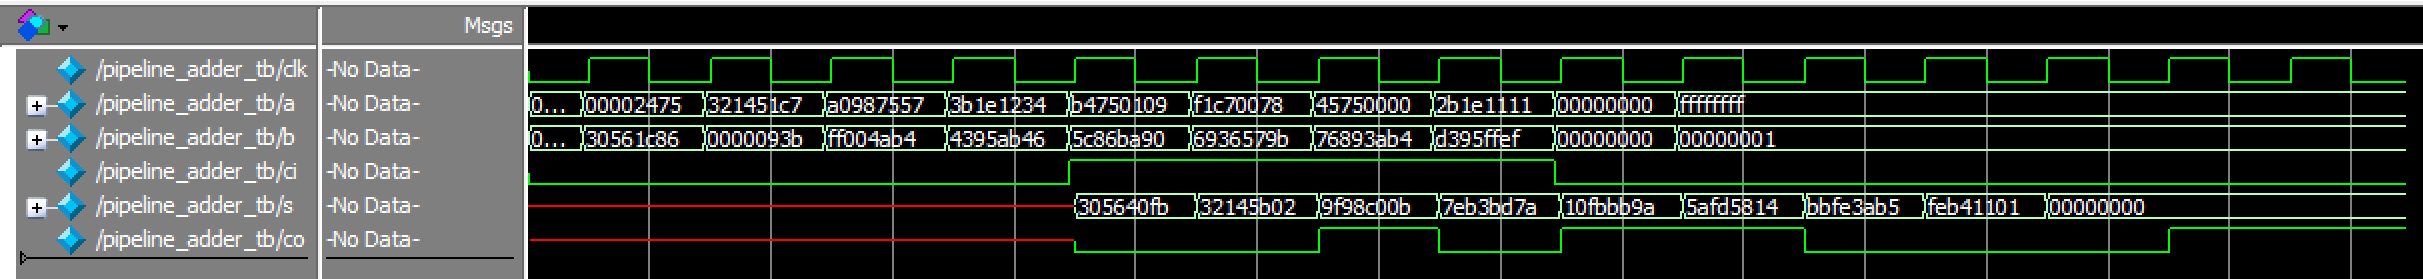
\includegraphics[width=1\textwidth]{p5.png}
    \caption{32位流水线加法器ModelSim仿真结果}
\end{figure}

后来发现，这是由于在第一个时钟上升沿（50ns）到来之前，a 和 b 的值就已经在 45ns 时刻被修改了。
因此，流水线根本没有机会采到初始的 0 值。它在第一个周期锁存的就是 32'h00002475 和 32'h30561c86。所以，在波形上永远看不到 0+0 的计算结果 00000000
\begin{lstlisting}[language=verilog, caption=pipeline\_adder\_tb.v]
initial begin clk=0; forever #(DELY/2) clk=~clk ;end
initial begin
       a=32'h00000000; b=32'h00000000;ci=0;
#45    a=32'h00002475; b=32'h30561c86;ci=0;
\end{lstlisting}
\begin{figure}[H]
    \centering
    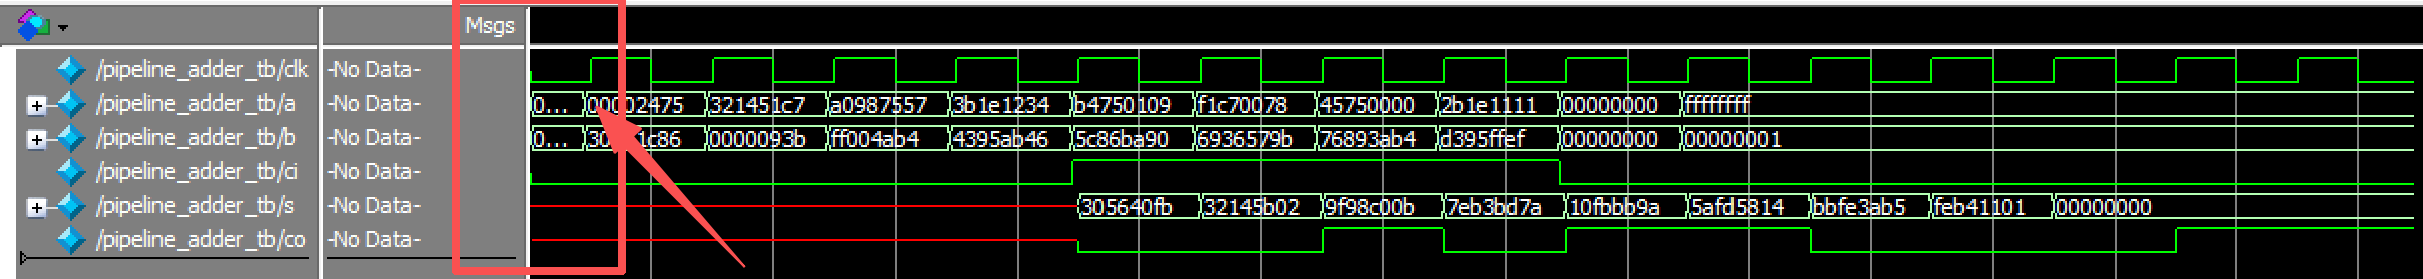
\includegraphics[width=1\textwidth]{p8.png}
    \caption{32位流水线加法器ModelSim仿真结果}
\end{figure}

基于此，将45ns改至50ns之后的55ns，流水线就能采到初始的 0 值。在波形上就能看到 0+0 的计算结果 00000000
\begin{lstlisting}[language=verilog, caption=pipeline\_adder\_tb.v]
initial begin clk=0; forever #(DELY/2) clk=~clk ;end
initial begin
       a=32'h00000000; b=32'h00000000;ci=0;
#55    a=32'h00002475; b=32'h30561c86;ci=0;
\end{lstlisting}

\begin{figure}[H]
    \centering
    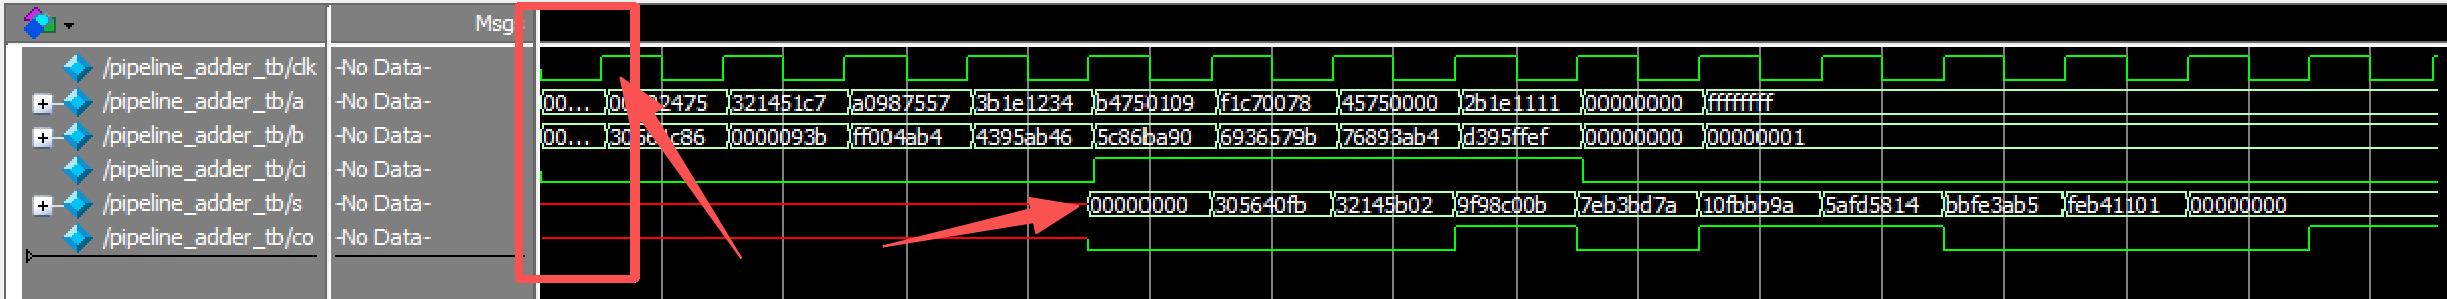
\includegraphics[width=1\textwidth]{p9.png}
    \caption{32位流水线加法器ModelSim仿真结果}
\end{figure}

同时，意识到，可能在原本的tb代码中，0值只是为了初始化a与b,45ns时刻修改a和b的值就是为了让流水线在第一个周期就能锁存到非0的值，

\section{\heiti\bfseries 思考题}

\begin{enumerate}
    \item 为什么要进行时序仿真？
    
    {\heiti\bfseries 答：}时序仿真在功能仿真的基础上，考虑了实际电路中的{\heiti\bfseries 延迟}因素，能够更真实地反映电路的实际工作情况。
    \begin{itemize}
        \item {\heiti\bfseries 验证时序约束：}检验设计是否满足建立时间（setup time）和保持时间（hold time）等时序要求，确保电路在目标时钟频率下能够正常工作。
        \item {\heiti\bfseries 发现竞争冒险：}功能仿真假设门电路无延迟，无法发现由于延迟差异导致的竞争冒险（race condition）和毛刺（glitch）等问题。
        \item {\heiti\bfseries 评估性能指标：}通过时序仿真可以准确测量电路的最大工作频率、关键路径延迟等性能参数，为优化设计提供依据。
    \end{itemize}
    
    \item 采用流水线技术有什么优缺点？

    {\heiti\bfseries 答：}
    
    {\heiti\bfseries 优点：}
    \begin{itemize}
        \item {\heiti\bfseries 提高系统工作频率：}将长延迟的组合逻辑分割成多个较短的阶段，每个阶段的延迟减小，可以使用更高的时钟频率。
        \item {\heiti\bfseries 提高吞吐量：}虽然单个数据的处理时间可能增加（由于寄存器延迟），但多个数据可以同时在不同流水线阶段处理，整体吞吐量大幅提升。
        \item {\heiti\bfseries 提高资源利用率：}各个流水线阶段可以并行工作，充分利用硬件资源，避免资源闲置。
        \item {\heiti\bfseries 降低功耗：}在相同吞吐量下，流水线设计可以使用较低的工作电压，从而降低功耗。
    \end{itemize}

   {\heiti\bfseries 缺点：}
    \begin{itemize}
        \item {\heiti\bfseries 增加硬件开销：}需要在各级之间插入寄存器（触发器），增加了硬件资源消耗和芯片面积。
        \item {\heiti\bfseries 增加延迟（Latency）：}虽然吞吐量提高了，但单个数据从输入到输出的总时间增加，因为需要经过多个时钟周期。
        \item {\heiti\bfseries 流水线冒险：}存在数据冒险、控制冒险等问题，可能需要额外的硬件（如前递单元、冲突检测）或软件（如插入空泡）来解决。
        \item {\heiti\bfseries 负载不均衡：}如果各级流水线的延迟差异较大，整体性能将受限于最慢的一级，导致其他级资源浪费。
        \item {\heiti\bfseries 初始化和填充开销：}流水线启动时需要若干周期才能填满，在处理少量数据时优势不明显。
    \end{itemize}
\end{enumerate}

\end{document}